\chapter[Planejamento]{Planejamento}
\label{cap:planejamento}

Antes de iniciar o desenvolvimento do projeto, foi necessário especificar os recursos necessários para a montagem do sistema, assim como a forma em que eles serão utilizados.
Esta seção descreve a escolha do equipamento e o projeto inicial do sistema.

\section[Escolha do equipamento]{Escolha do equipamento}
\label{sec:escolhaEquipamento}

Para o desenvolvimento do projeto, foram disponibilizados, pela instituição CEFET-MG, dois manipuladores robóticos e diversos dispositivos que podem ser utilizados para seu controle.
A partir desse equipamento, e de outros disponíveis no mercado, foi decidido como o projeto seria realizado.
Os equipamentos utilizados para o projeto estão descritos a seguir:

\subsection[Manipuladores]{Manipuladores}

Os principais elementos deste trabalho são os manipuladores robóticos, portanto foi feito inicialmente um estudo sobre seu funcionamento e sobre como seu controle pode ser realizado para movimentar as peças de xadrez.

Foi disponibilizado um manipulador robótico de modelo Mentor de cor preta, conforme a figura \ref{fig:fotoManipuladorMentor}, e um manipulador de modelo RD5NT de cor azul, conforme a figura \ref{fig:fotoManipuladorAzul}.
Esses manipuladores possuem características diferentes, portanto seu controle deve ser realizado de forma diferente.
Eles possuem diversas juntas movimentadas por motores de corrente contínua, e permitem que o manipulador funcione de forma similar a um braço humano.
Além disso, cada junta possui um potenciômetro que indica a posição atual do eixo, por meio de um sinal analógico.

O manipulador Mentor apresenta 5 graus de liberdade e um \textit{gripper} que pode ser utilizado para pegar e soltar objetos.
Além disso, ele possui caixas de redução em seus motores, o que permite que ele mantenha sua posição mesmo após o desligamento dos motores.
Suas dimensões e faixas de movimento são apresentadas na tabela \ref{tab:caracteristicasManipuladorMentor} \cite{mentor_forward_kinematics}.

Já o manipulador RD5NT possui apenas 4 graus de liberdade e um \textit{gripper}.
Ele não possui caixas de redução, o que faz com que ele perca sua posição quando os motores são desligados.
Portanto, seu controle deve ser realizado de forma contínua, para que ele permaneça na posição desejada.
Suas dimensões e faixas de movimento são apresentadas na tabela \ref{tab:caracteristicasManipuladorRD5NT} \cite{controle_neural_robo}.

\begin{table}
    \centering
    \caption{Características do manipulador robótico Mentor}
    \label{tab:caracteristicasManipuladorMentor}
    \begin{tabular}{|l|l|l|}
        \hline
        \textbf{Eixo} & \textbf{Movimento angular (graus)} & \textbf{Comprimento (mm)} \\ \hline
        \textbf{Eixo 0 (\textit{Waist})}            & 210 & 185 \\ \hline
        \textbf{Eixo 1 (\textit{Shoulder})}         & 180 & 165 \\ \hline
        \textbf{Eixo 2 (\textit{Elbow})}            & 230 & 150 \\ \hline
        \textbf{Eixo 3 (\textit{Left Wrist Axle})}  & 320 & 0 \\ \hline
        \textbf{Eixo 4 (\textit{Right Wrist Axle})} & 320 & 0 \\ \hline
        \textbf{\textit{Wrist Pitch}}               & 140 & - \\ \hline
        \textbf{\textit{Wrist Roll}}                & 320 & - \\ \hline
    \end{tabular}
\end{table}

\begin{table}
    \centering
    \caption{Características do manipulador robótico RD5NT}
    \label{tab:caracteristicasManipuladorRD5NT}
    \begin{tabular}{|l|l|l|}
        \hline
        \textbf{Eixo} & \textbf{Movimento angular (graus)} & \textbf{Comprimento (mm)} \\ \hline
        \textbf{Eixo 0 (\textit{Waist})}            & 293 & 110 \\ \hline
        \textbf{Eixo 1 (\textit{Shoulder})}         & 107 & 120 \\ \hline
        \textbf{Eixo 2 (\textit{Elbow})}            & 284 & 160 \\ \hline
        \textbf{Eixo 3 (\textit{Wrist Axle})}       & 360 & 0 \\ \hline
    \end{tabular}
\end{table}

\begin{figure}[H]
    \begin{minipage}{.5\textwidth}
        \centering
        \caption{Manipulador Robótico Mentor}
        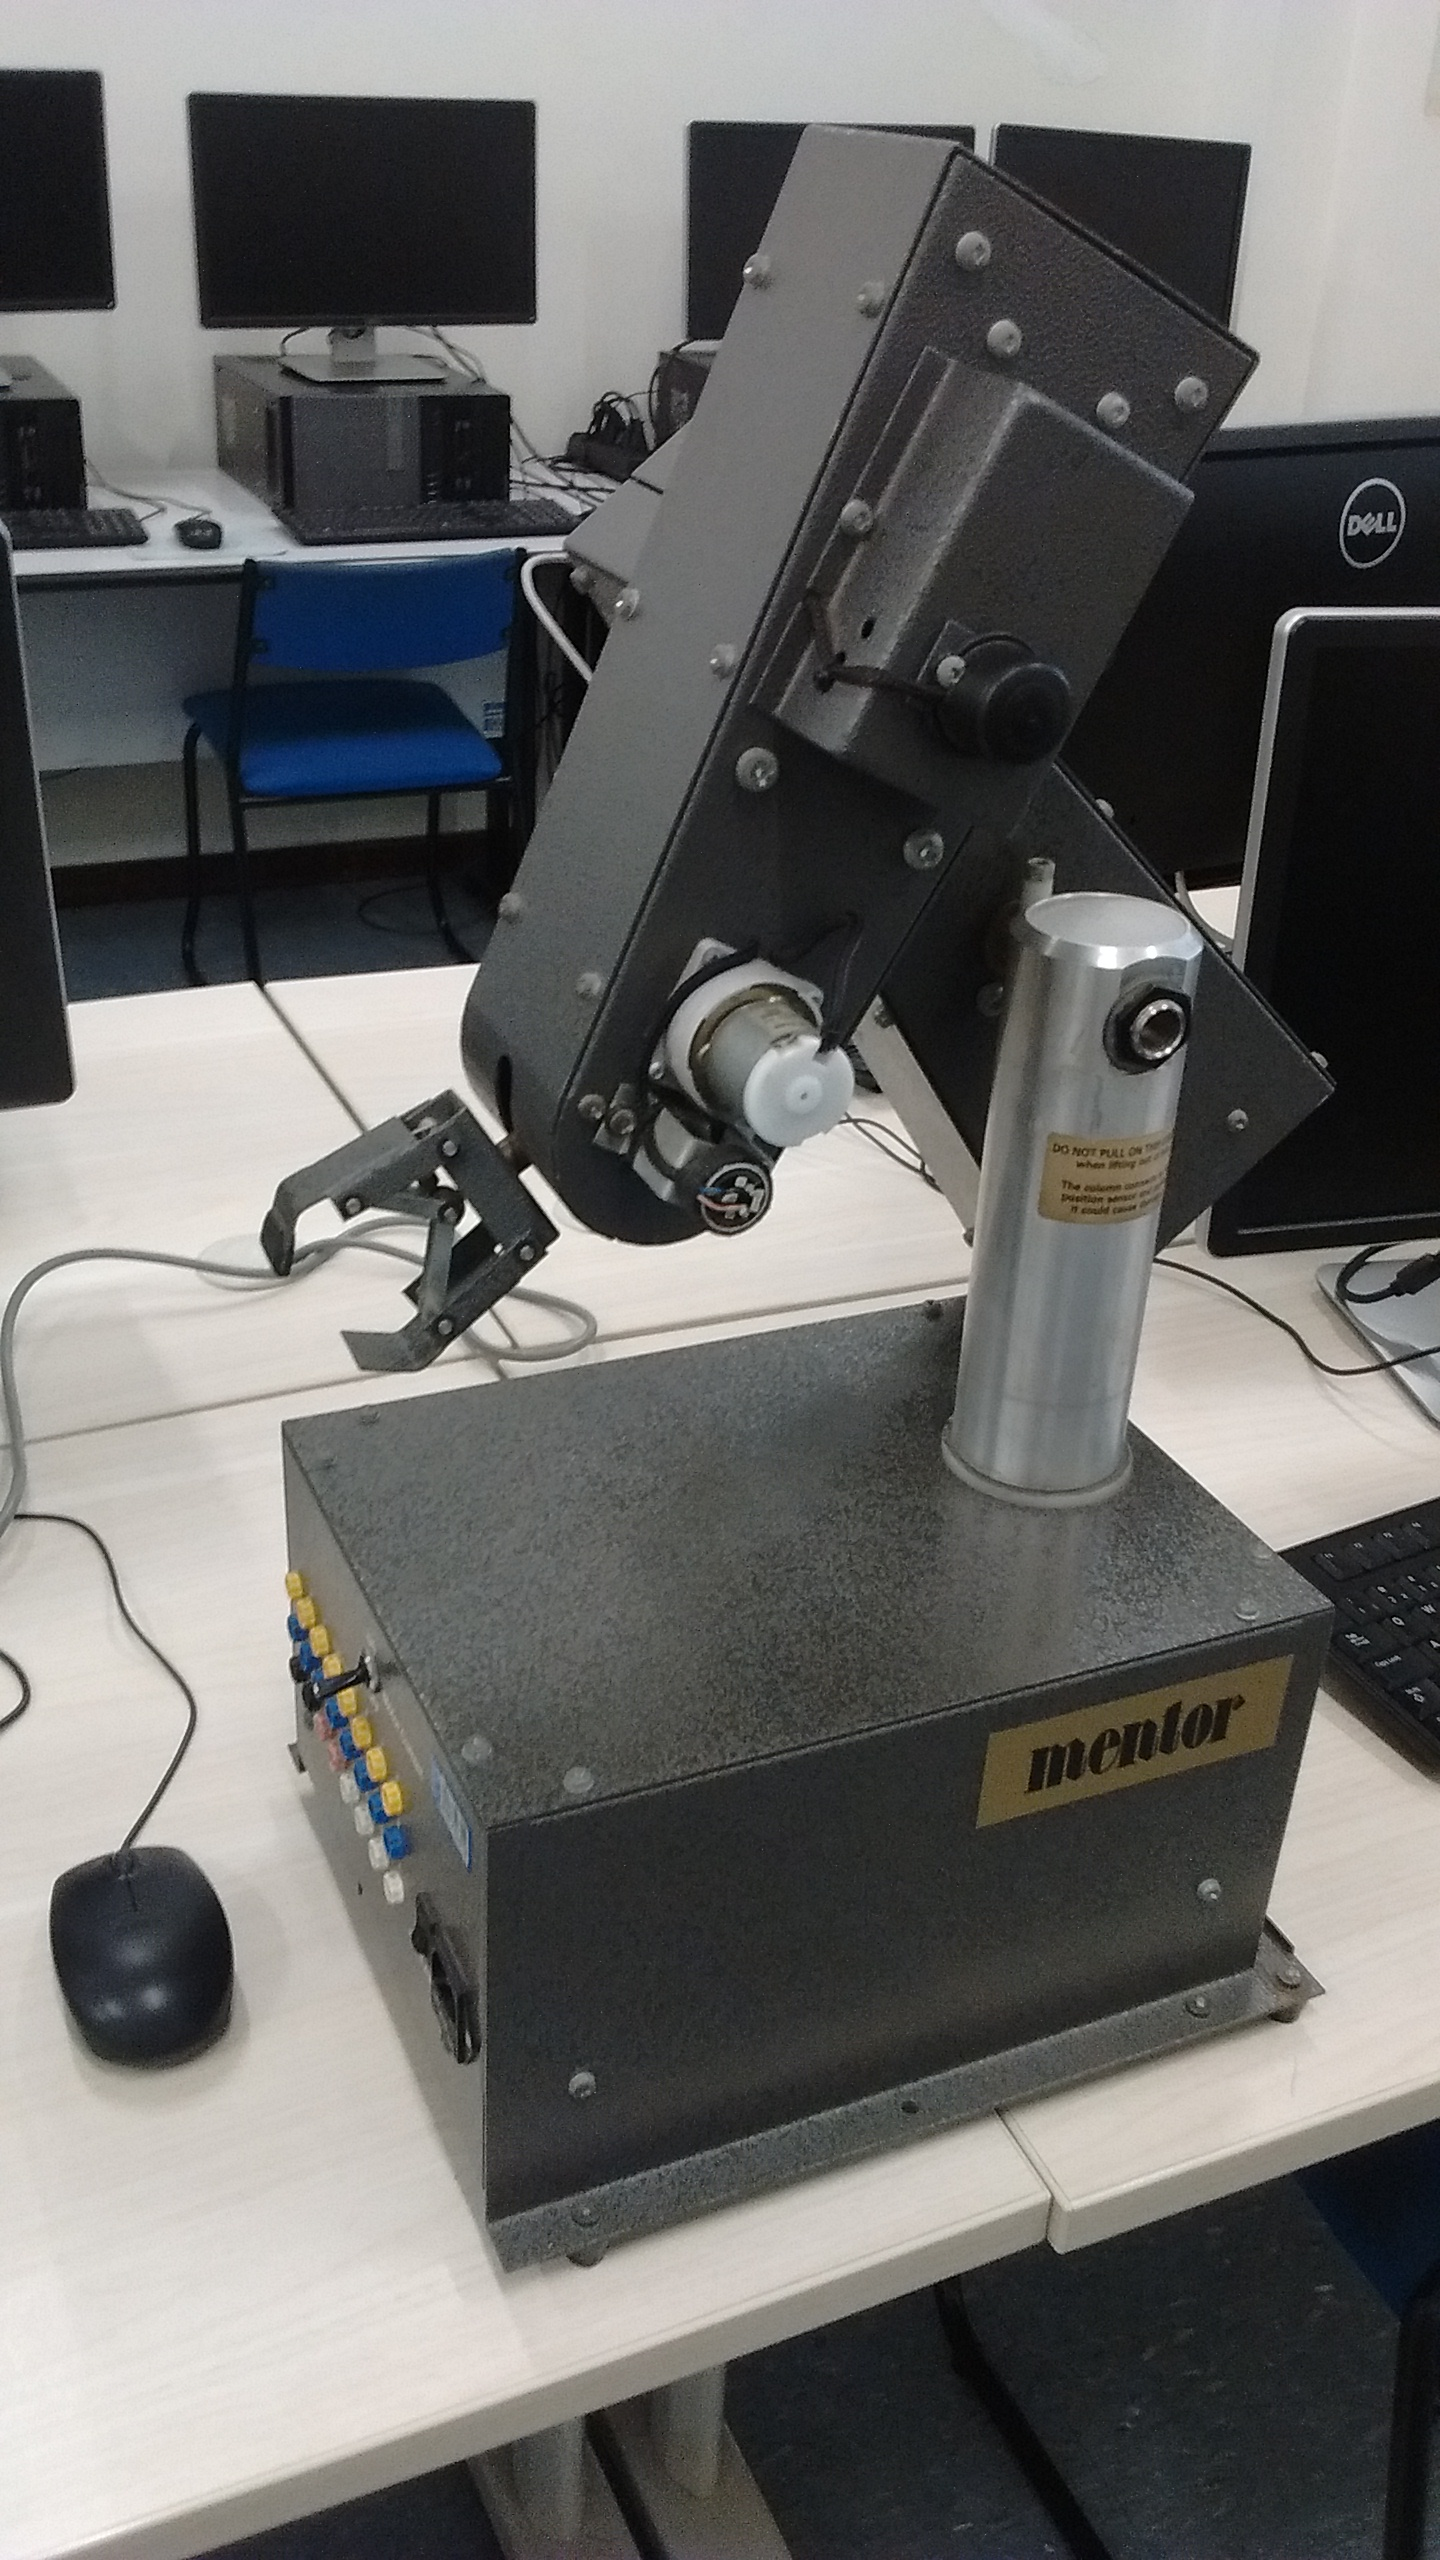
\includegraphics[keepaspectratio=true, width=0.9\linewidth]
            {img/foto-manipulador-preto.jpg}
        \fonte{http://arquivo.eng.br/robotica}
        \label{fig:fotoManipuladorMentor}
    \end{minipage}
    \begin{minipage}{.5\textwidth}
        \centering
        \caption{Manipulador Robótico Azul}
        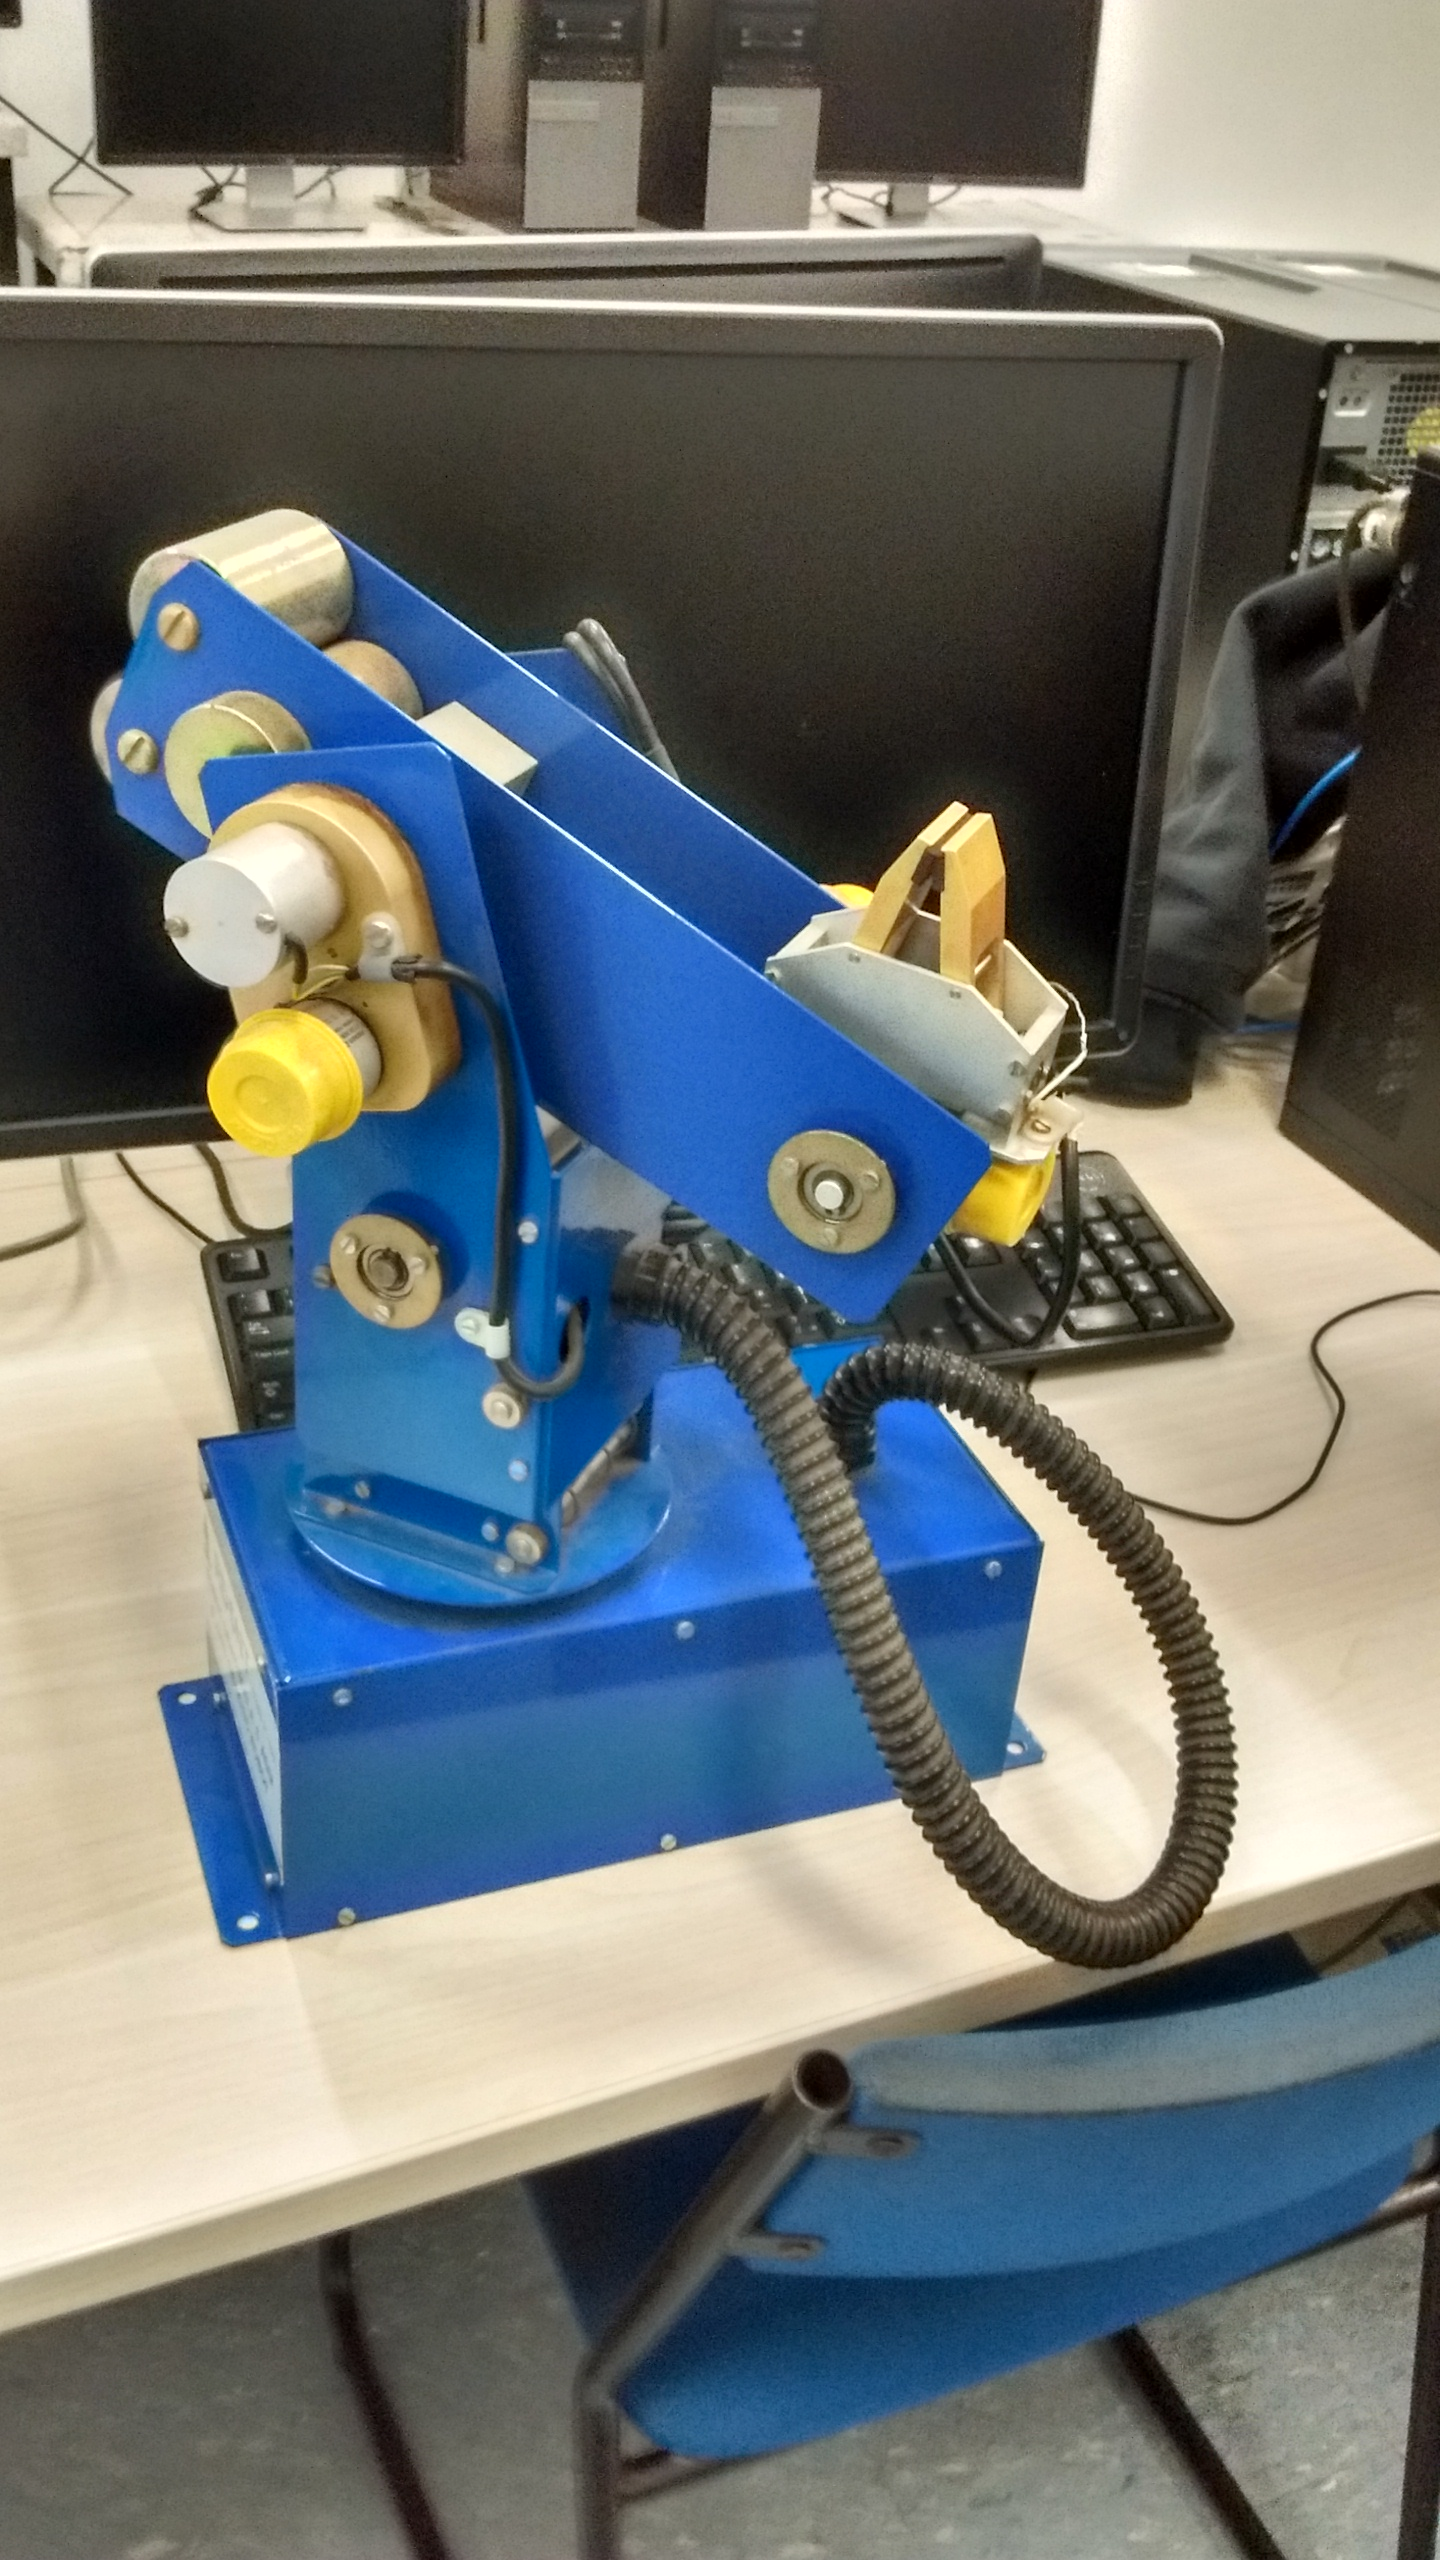
\includegraphics[keepaspectratio=true, width=0.9\linewidth]
            {img/foto-manipulador-azul.jpg}
        \fonte{http://arquivo.eng.br/robotica}
        \label{fig:fotoManipuladorAzul}
    \end{minipage}%
\end{figure}

\subsection[Manete para os jogadores]{Manete para os jogadores}
\label{sub:maneteJogadores}

Para que os jogadores possam interagir com os manipuladores, foi utilizado uma manete de modelo \textit{batpad}, que possui dois \textit{joysticks}, conforme a figura \ref{fig:fotoManeteJogadores}.
Cada um desses \textit{joysticks} deve ser alimentado com 5V e envia sinais que indicam sua posição nos eixos X e Y, além de um botão que pode ser pressionado.

Os sinais de posição são enviados de forma analógica, com valores de tensão que variam de 0V a 5V.
O sinal do botão é enviado de forma digital, com valores de tensão de 0V ou 5V, sendo que 0V indica que o botão está pressionado.

Cada jogador possui uma manete para controlar um dos manipuladores robóticos.

\begin{figure}[H]
    \centering
    \caption{Manete para os jogadores}
    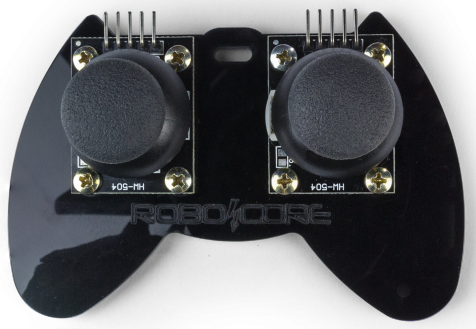
\includegraphics[keepaspectratio=true, width=0.5\textwidth]
    	{img/foto-controle-jogadores.png}
    \fonte{https://www.robocore.net/acessorios-robocore/controle-batpad}
    \label{fig:fotoManeteJogadores}
\end{figure}

\subsection[Microcontrolador]{Microcontrolador}
\label{sub:microcontrolador}

Para realizar a integração entre a manete e os manipuladores, foi utilizado um microcontrolador Arduino Mega 2560, conforme a figura \ref{fig:fotoArduino}.
Esse microcontrolador possui um \textit{clock} de 16MHz, 256KB de memória \textit{flash}, 8KB de memória \textit{RAM} e 4KB de memória \textit{EEPROM}.
Ele apresenta 16 entradas analógicas e 54 entradas e saídas digitais, sendo que 15 delas podem ser utilizadas como saídas \textit{PWM}  \cite{arduino_mega_2560_datasheet}.

Cada microcontrolador é responsável por controlar um dos manipuladores robóticos.
Ele realiza a leitura dos sinais analógicos e digitais provenientes da manete, que se referem à posição atual do \textit{joystick} e o estado do botão, e a leitura de sinais analógicos provenientes do manipulador robótico, que indicam a posição atual de cada junta.
A partir desses sinais, ele realiza o cálculo das posições desejadas de cada junta do manipulador e envia sinais de controle para elas.

Os sinais de controle são digitais do tipo \textit{PWM} (\textit{Pulse Width Modulation}), que variam de 0V a 5V, para possibilitar o controle da velocidade de rotação dos motores através da variação da largura do pulso.
Valores maiores de \textit{Duty Cycle} [Ciclo de Trabalho] resultam em maior velocidade de rotação do motor, pois o sinal permanece em nível alto por um período maior de tempo.
Por outro lado, valores menores de \textit{Duty Cycle} resultam em menor velocidade de rotação do motor, pois o sinal permanece em nível alto por um período menor de tempo.
Para definir o sentido de rotação do motor, foi utilizado um sinal digital que indica se ele deve girar no sentido horário ou anti-horário.

Por fim, o microcontrolador é conectado a um computador através de um cabo USB.
O Arduino é responsável por comunicar com o computador quais os movimentos que o jogador deseja realizar com seu manipulador robótico.
A partir disso, o computador responde se o movimento é permitido ou não.

\begin{figure}[H]
    \centering
    \caption{Largura do pulso do sinal de controle}
    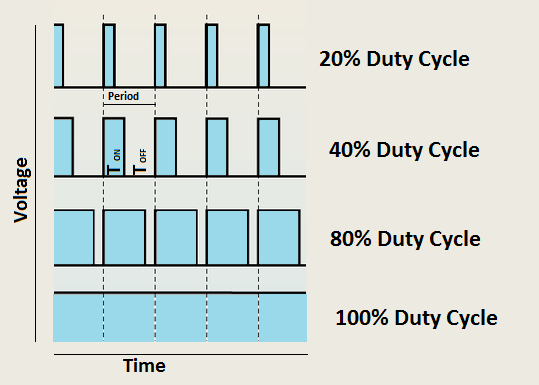
\includegraphics[keepaspectratio=true, width=0.5\textwidth]
    	{img/pwm.png}
    \fonte{https://create.arduino.cc/projecthub/muhammad-aqib/arduino-pwm-tutorial-ae9d71}
    \label{fig:pwm}
\end{figure}

\begin{figure}[H]
    \centering
    \caption{Microcontrolador Arduino Mega 2560}
    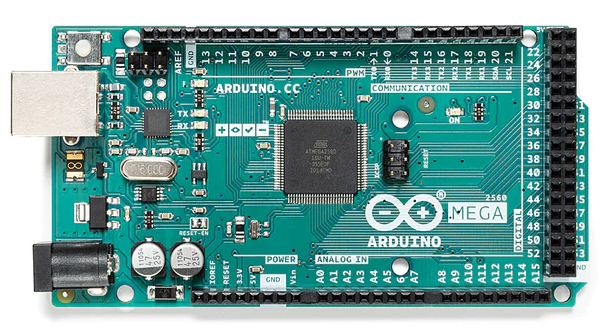
\includegraphics[keepaspectratio=true, width=0.5\textwidth]
    	{img/foto-arduino.png}
    \fonte{https://store.arduino.cc/products/arduino-mega-2560-rev3}
    \label{fig:fotoArduino}
\end{figure}

\subsection[Placa de Controle]{Placa de Controle}
\label{sub:placaControle}

Para controlar os motores dos manipuladores, é necessário o uso de uma placa de controle para converter os sinais de baixa potência provenientes do Microcontrolador em sinais de maior potência que movimentam as juntas dos manipuladores robóticos.
Essa placa é alimentada com 12v e ela recebe os sinais digitais de direção e de \textit{PWM} do Arduino e movimenta os motores de acordo.

Para obter essa funcionalidade, foi feito o uso de módulos de ponte H, similar aos utilizados na placa apresentada na figura \ref{fig:ponteH}.
Uma ponte H é um Circuito Integrado (CI) utilizado para aplicar uma tensão variável a um componente através de um sinal de \textit{PWM}.
Ela também permite alterar a direção em que a corrente é aplicada no componente, o que possibilita inverter o sentido de rotação de um motor \cite{h_bridge}.


\begin{figure}[H]
    \centering
    \caption{Módulo de Ponte H}
    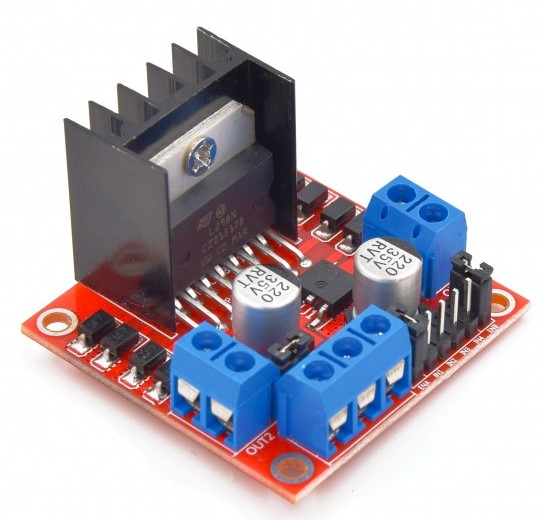
\includegraphics[keepaspectratio=true, width=0.5\textwidth]
    	{img/ponte-h.jpg}
    \fonte{https://www.smart-prototyping.com/L298N-Dual-H-bridge-Motor-Driver-Board}
    \label{fig:ponteH}
\end{figure}

\subsection[Computador]{Computador}
\label{sub:computador}

Para gerenciar o jogo, foi necessário o uso de um computador.
Ele é responsável por receber realizar a comunicação com o microcontrolador para gerenciar o jogo de Xadrez.

Para comunicar com o Arduino, é utilizado um cabo USB e comunicação serial.
A comunicação serial é um protocolo de comunicação assíncrona que permite a transmissão de dados entre dois dispositivos.
Nesse caso, o Arduino envia o movimento desejado pelo jogador e o computador responde se o movimento é permitido ou não.

A verificação do movimento é feita através de um algoritmo que implementa a lógica do jogo de Xadrez.
Através dele, são avaliadas as regras de movimentação de cada peça, as regras de captura e de xeque.
Também são verificadas as regras de xeque-mate e de empate por falta de material.
Com base nessas regras e no estado atual do tabuleiro, o computador responde se o movimento é permitido ou não.

\section[Projeto do sistema]{Projeto do sistema}
\label{sec:projetoSistema}

Após a definição de todos os equipamentos a serem utilizados, foi feito o projeto do sistema.
Esse projeto consiste na definição de como os dispositivos serão interligados e como o sistema irá funcionar.

A manete deve ser alimentada com 5V e ser conectada ao Arduino para permitir a leitura dos sinais de entrada.
Essa conexão é realizada com 10 cabos, sendo 5 para cada \textit{joystick} com seu respectivo botão.

A placa de controle deve ser alimentada com 12V e também deve ser conectada ao Arduino para receber os sinais de controle.
Essa conexão é realizada com 10 cabos, 2 para o controle de cada junta do manipulador robótico.
Essa placa também deve ser conectada aos motores do manipulador robótico, também com 10 cabos, 2 para cada junta.

O manipulador robótico deve ser conectado ao Arduino para o envio dos sinais de posição de cada junta.
Essa conexão é realizada com 5 cabos, um para cada junta.

Por fim, o Arduino deve ser alimentado com 5V e deve ser conectado a um computador para a implementação da lógica do jogo.

A montagem do sistema é mostrada na Figura \ref{fig:montagemSistema}.

\begin{figure}[H]
    \centering
    \caption{Montagem do Sistema}
    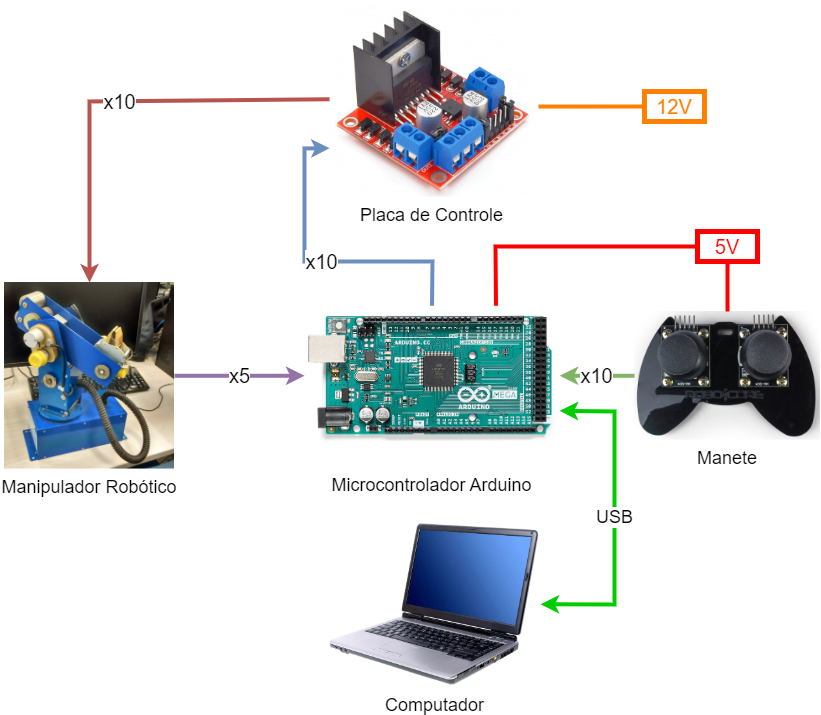
\includegraphics[keepaspectratio=true, width=0.8\textwidth]
    	{img/projeto-sistema.png}
    \fonte{Do próprio autor}
    \label{fig:montagemSistema}
\end{figure}


